\subsection{JPEG}
JPEG představuje jeden z nejpoužívanějších obrazových formátů (fotografie), jedná se o \textbf{ztrátový} formát obrázků. \textbf{Komprese JPEG} pracuje v několika krocích, principem je \textbf{redukce vysokofrekvenčních dat} v obrázků při zachování co nejvíce informací o nízkofrekvenčních datech. To je založeno na tom, že lidské oko se zaměřuje spíše na nízké frekvence (malou změnu jasu na ploše) a vysoké frekvence vnímá hůře (hrany). Můžeme si je tedy dovolit redukovat bez znatelné ztráty kvality obrazu. Zároveň se využívá \textbf{podvzorkování barev} $\rightarrow$ znovu z toho důvodu, že lidské oko vnímá více jas než barvy.

\begin{figure}[H]
	\centering
	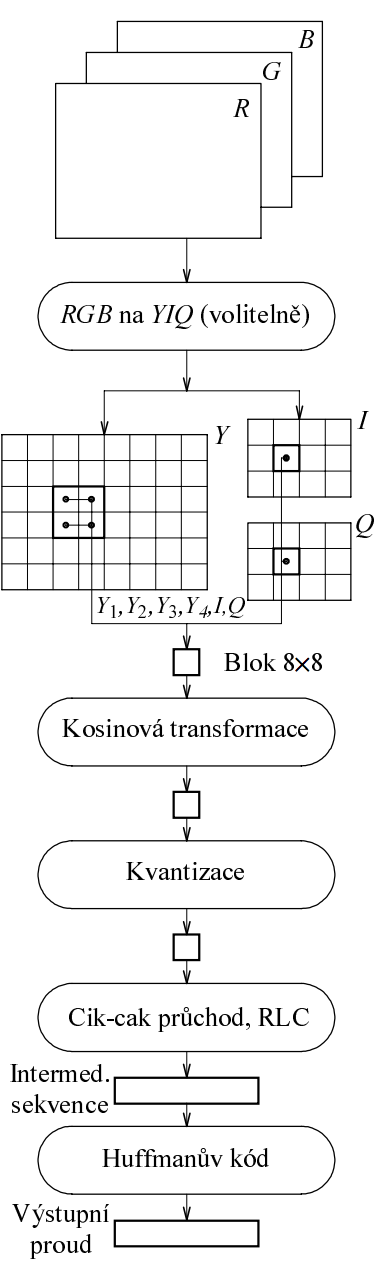
\includegraphics[width=0.3\textwidth]{assets/7_jpeg}
\end{figure}

\subsubsection{Komprese JPEG}
\begin{enumerate}
	\item \textbf{Převod RGB na YCbCr} -- vstupní obraz se převede na YCbCr, což jej rozdělí na \textbf{jasovou složku} (Y) a \textbf{chrominanční} složky (barvonosné Cb a Cr). To nám umožňuje následnou redukci barvonosné složky v jednom ze 3 módů: 4:4:4 (nepodvzorkovává se), 4:2:2 (horizontálně na polovinu, pro 2 jasové 1 barva), 4:2:0 (horizontálně i vertikálně na polovinu, pro 4 jasové 1 barva).
	\item \textbf{Provedení DCT} -- obraz se následně rozdělí na bloky o velikosti $8 \times 8$. Pro každý blok se provede 2D DCT (diskrétní kosinova transformace), ta narozdíl od DFT produkuje pouze reálné komponenty. Výsledek DCT nám vrátí počet jednotlivých frekvencí, které se v obraze nachází, přičemž \textbf{nízké frekvence} se koncentrují vlevo nahoře a \textbf{vysoké frekvence} vpravo dole (viz obrázek).
	\begin{figure}[H]
		\centering
		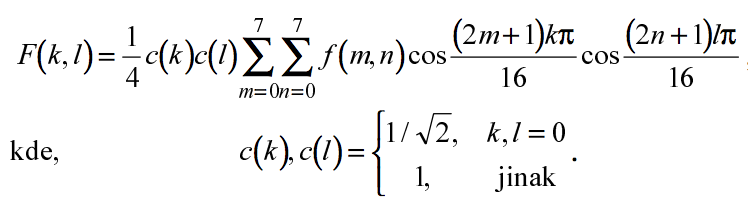
\includegraphics[width=0.8\textwidth]{assets/7_dct1}
		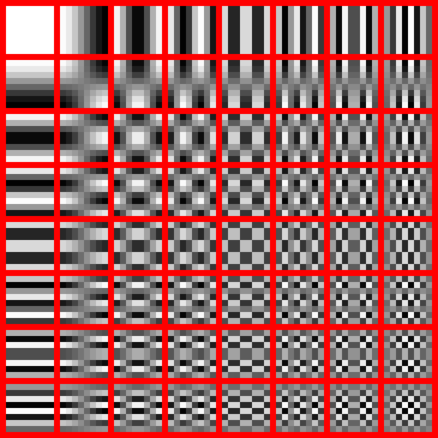
\includegraphics[width=0.3\textwidth]{assets/7_dct2}
		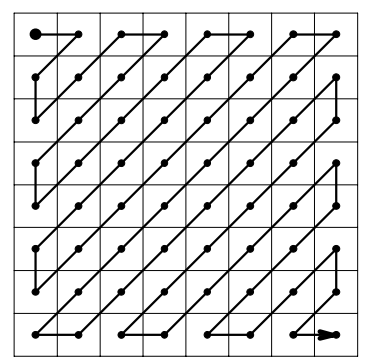
\includegraphics[width=0.35\textwidth]{assets/7_jpeg_zigzag}
	\end{figure}
	\item \textbf{Kvantizace} -- jednotlivé bloky jsou \textbf{vyděleny kvantizační maticí a zaokrouhleny}. Koeficienty matice definují \textbf{míru komprese} (čím větší hodnoty tím větší komprese a horší obraz). Většinou po aplikaci kvantizace v každém bloku zůstane pouze několik hodnot \textbf{vlevo nahoře} to vyplývá z toho co jsme zmínil výše $\rightarrow$ více se redukují vysoké frekvence, které si můžeme dovolit vynechat. Výsledek před a po kvantizaci je vidět obrázku níže.
	\begin{figure}[H]
		\centering
		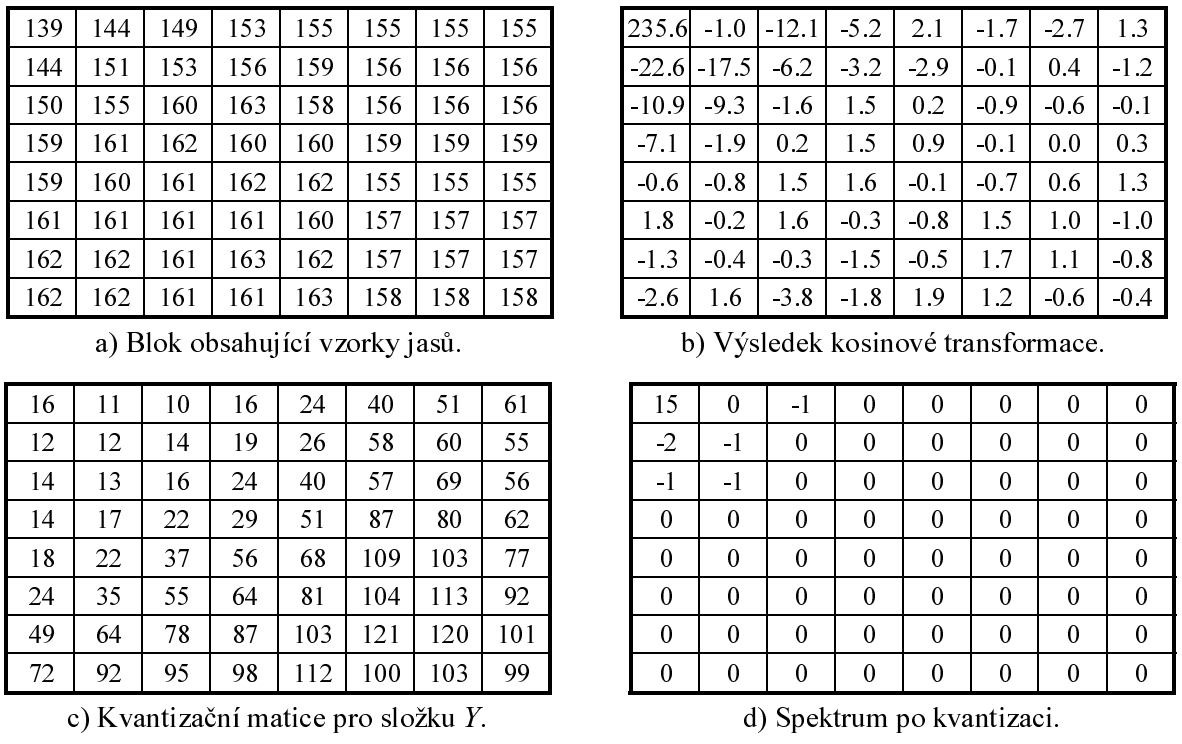
\includegraphics[width=0.8\textwidth]{assets/7_kvantizace}
	\end{figure}
	\item \textbf{Zig-zag intermediální sekvence} -- obraz po kvantizaci se projde \textbf{zig-zagem} a z daných čísel se vytvoří intermediální sekvence (\textbf{dvojice} ve tvaru \textbf{Symbol-1}, \textbf{Symbol-2}) pomocí \textbf{Run-Length encoding}. RLE kóduje pouze AC složky (1 - 64), DC složka (px na souřadnicích [0, 0] každého bloku) se kóduje \textbf{diferenciálně} vzhledem k DC složce v předchozím bloku. Intermediální sekvence vypadá následovně:
	\begin{itemize}
		\item \textbf{Symbol-2} -- (AMPLITUDE) značí hodnotu na daném pixelu po kvantizaci.
		\item \textbf{Symbol-1} -- (RUNLENGTH, SIZE), kde RUNLENGTH značí počet nul, které danému prvku předchází v zig-zag sekvenci (pokud je počet větší než 15, zapíše se 15) a SIZE je počet bitů nutných k reprezentaci AMPLITUDE. \textbf{Speciální hodnota} (0, 0) říká, že předchozí nenulová hodnota byla poslední.
		\item \textbf{Kódování} -- \textbf{DC} složky se kódují odlišně (SIZE, AMPLITUDE), \textbf{AC} složky ((AMPLITUDE), (RUNLENGTH, SIZE).
	\end{itemize}
	Intermediální sekvence se poté zakóduje \textbf{Huffmanovým kódem}, kde se kódují pouze kombinace (RUNLENGTH, SIZE) u AC a (SIZE) u DC podle předem daných tabulek. AMPLITUDE se zapisuje pomocí \textbf{jednotkového doplňku} (způsob reprezentace záporných čísel).
	\begin{figure}[H]
		\centering
		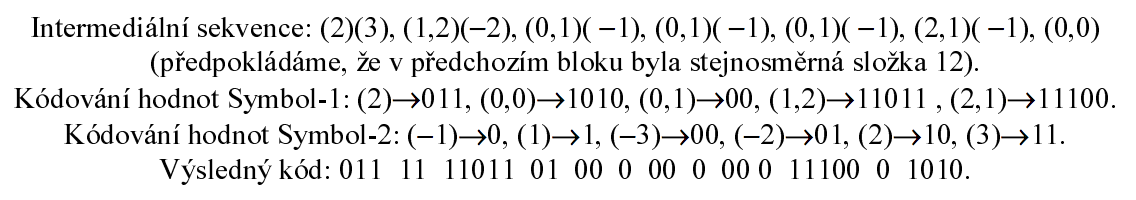
\includegraphics[width=\textwidth]{assets/7_intermediate}
	\end{figure}
\end{enumerate}

\subsection{MPEG}
MPEG je zkratkou pro Moving Picture Expert Group. Cílem práce této skupiny bylo standardizovat metody komprese videosignálu. Existuje několik standardů MPEG-(1, 2, 4, 7). 

\begin{figure}[H]
	\centering
	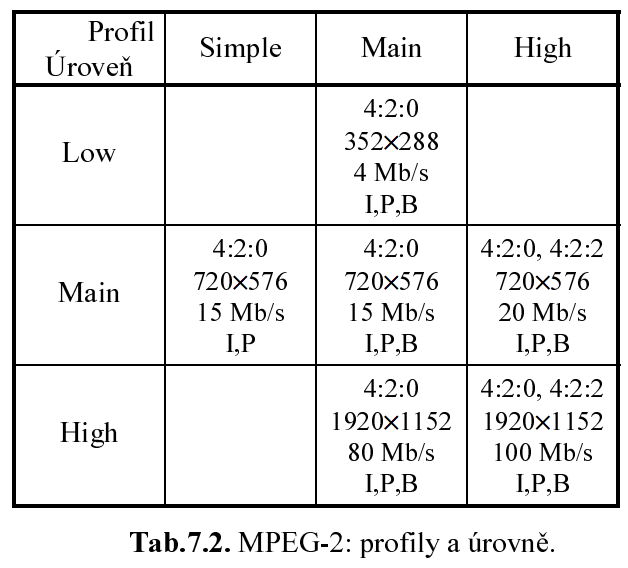
\includegraphics[width=0.5\textwidth]{assets/7_mpeg}
\end{figure}

\begin{itemize}
\item \textbf{MPEG-1} -- první standard, dokončen v roce 1991. Navržen zejména pro práci s obrazy $352\times288$ pixelů, 25FPS (odvozeno od televizní normy PAL) nebo $352\times240$, 30FPS (odvozeno od NTSC) při datovém toku \textbf{1.5 MBit/s} (optimální tok, mohl být i vyšší).
\item \textbf{MPEG-2} -- dokončen v roce 1994, mnohem velkorysejší implementace, snaží se být co \textbf{nejuniverzálnější}. Zavádí několik \textbf{profilů} (podmnožina z nejširší možné syntaxe) a \textbf{úrovní} (definuje parametry v rámci daného profilu).
\item \textbf{MPEG-3} -- práce na tomto standardu byly zastaveny (měl sloužit pro HDTV) později byl sloučen do MPEG-2.
\item \textbf{MPEG-4} -- metodou komprese se značně liší oproti MPEG-1,2, je určen pro \textbf{extrémně nízké datové toky}.
\item \textbf{MPEG-7} -- neříká nic o kódování, jedná se o standard pro popis dat (\textbf{metadata}) s multimediálním obsahem.
\end{itemize}

\subsubsection{Komprese MPEG}
Standard MPEG, rozlišuje \textbf{tři typy rámců (I, B, P)},  ve své podstatě pro kódování využívá stejných principů jako JPEG (\textbf{rámec I} se kóduje nezávisle). Oproti JPEG však využívá i \textbf{časové koherence}. Tedy k dosažení maximální komprese se předpokládá, že po sobě jdoucí rámce jsou s největší pravděpodobností dosti podobné. Počítá se ovšem s tím, že části obrazů se mohou přemístit, k tomu se využívá vložených rámců P a B, které se kódují \textbf{závisle} vzhledem k ostatním.
\begin{itemize}
\item \textbf{I} -- jsou kódovány každý \textbf{zvlášť}, bez vazby na rámce předcházející či následující. Pricip kódování (komprese) je stejný jako u standardu \textbf{JPEG} (i když v detailech existují některé \textbf{odlišnosti}: jiná kvantovací tabulka, jiná struktura intermediální sekvence a jiný způsob \textbf{zig-zagu} (podle MPEG-2)). \textbf{Kvantizační tabulka} může být pro každý makroblok jiná -- změnou měřítka lze \textbf{řídit tok dat} (některé aplikace mohou vyžadovat konstantní tok dat).
\item \textbf{P (Predicted)} -- tento rámec je kódován \textbf{vzhledem k jedinému předcházejícímu rámci typu I nebo P}. 
\item \textbf{B (Interpolated bi-directionally)} -- tyto rámce jsou kódovány vzhledem k nejbližšímu \textbf{předchozímu} a \textbf{nejbližšímu} budoucímu rámci typu \textbf{I} nebo \textbf{P}. Jejich použití je nepovinné ale z hlediska dosahovaných kompresních poměrů výhodné. \textbf{Komplikace} z použití rámců B spočívá v uchovávání v paměti dva kotevní obrazy. Dále je nevyhnutelné jisté časové zpoždění, protože nejprve musí být k dispozici obraz \textbf{novější} a teprve potom může být kódován obraz starší.
\begin{figure}[H]
	\centering
	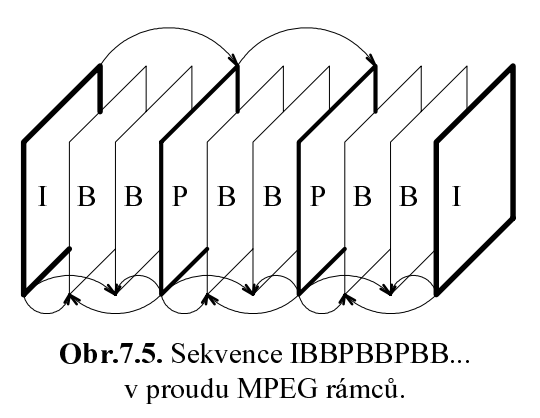
\includegraphics[width=0.48\textwidth]{assets/7_mpeg_komprese}
	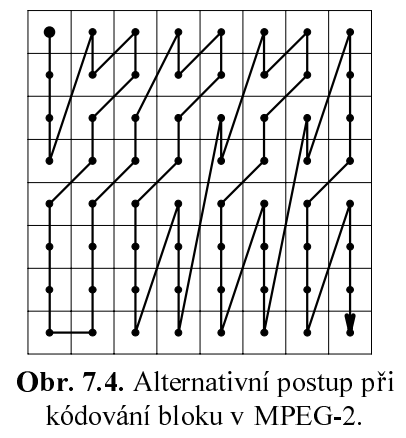
\includegraphics[width=0.35\textwidth]{assets/7_mpeg_zigzag}
\end{figure}
\end{itemize}

Velmi často používané řazení rámců je IBBPBBPBBI. Kódování rámců P a B taky probíhá po \textbf{makroblocích}. Pro každý makroblok v cílovém (tj. právě kódovaném rámci) jsou sestaveny \textbf{vektory pohybu} (pro každý makroblok v P \textbf{jeden} vektor, v B jsou vektory \textbf{dva}) vzhledem k referenčním rámcům.

\textbf{Vektor pohybu} je definován takto: jestliže o uvedený vektor posuneme kódovaný makroblok a porovnáme s odpovídající částí referenčního obrazu, pak je dosaženo dobré shody. Vektory posunutí se stávají \textbf{součástí komprimované} sekvence. Po nalezení vektoru jsou \textbf{kódovány diference} -- podobně jako u JPEGu mezi odpovídajícími makrobloky bude v dvou rámcích \textbf{malý rozdíl} a výsledné data po kvantizaci vyžadují tak \textbf{malé sekvence} (komprese).
\begin{itemize}
\item Bloky \textbf{P} se kódují $T-R$, kde T je makroblok v cílovém rámci,
\item bloky \textbf{B} se kódují $T - 0.5 (R_1 + R_2)$, kde $R_1$ a $R_2$ jsou makrobloky v cílových rámcích.
\end{itemize}

\begin{figure}[H]
	\centering
	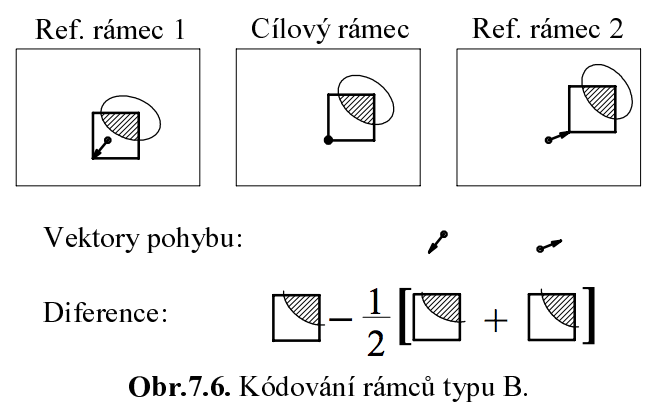
\includegraphics[width=0.48\textwidth]{assets/7_mpeg_kodovani_B}
\end{figure}

\subsubsection{Stanovení pohybového vektoru}
Stanovení pohybového vektoru MPEG norma nepředepisuje, jedná se však o jeden z \textbf{nejobtížnějších problémů}. Většinou se využívá pouze \textbf{jasové} (Y) složky, existuje několik metod:

\begin{enumerate}
\item \textbf{Porovnání makrobloků} -- v referenčním rámci se nalezne makroblok, který nejvíce odpovídá zpracovávanému makrobloku. Pro určení shody lze použít např. SSD. \textbf{Účinné}, avšak velmi \textbf{časově náročné}.
\item \textbf{Logaritmické vyhledávání} -- vylepšení předchozí metody, má logaritmickou časovou složitost. V prvním kroku algoritmus testuje 9 dvojic. V každém dalším kroku se testuje vždy po 8 dvojicích rozmístěných kolem předchozího bodu, který měl největší shodu. Rychlejší, ale nemusí být tak přesné jak předchozí metoda.
\item \textbf{Rekurzivní dělení} -- rekurzivně dělíme obraz na menší a menší. Poté nalezneme prvotní odhad v nejmenším obraze a se zvyšující se velikostí (návrat z rekurze) pozici vektoru jen upřesňujeme. Rychlé a spolehlivé.
\end{enumerate}

\begin{figure}[H]
	\centering
	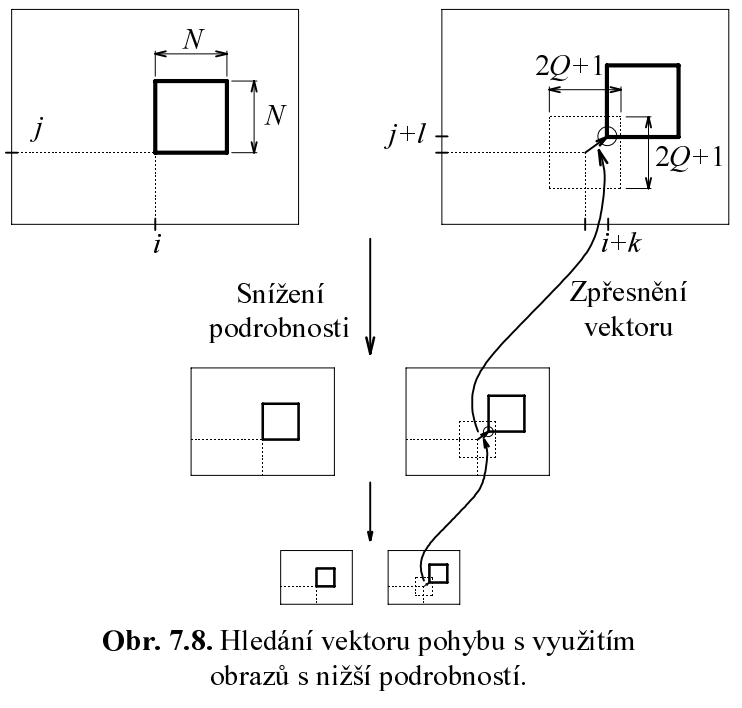
\includegraphics[width=0.48\textwidth]{assets/7_mpeg_rekurze}
	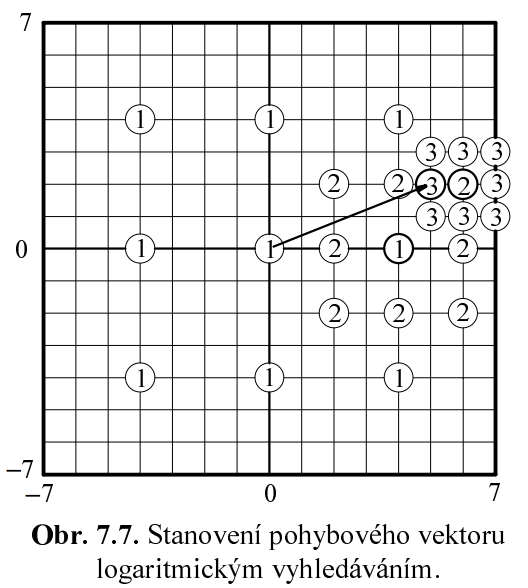
\includegraphics[width=0.48\textwidth]{assets/7_mpeg_log}
\end{figure}

Kódování složek vektorů se provádí \textbf{inkrementálně vzhledem k předchozí hodnotě}. Zároveň může nastat situace kdy se vektor nepodaří nalézt, v tom případě je možné kódovat dané makrobloky nezávisle na ostatních (stejně jako I).

\begin{figure}[H]
	\centering
	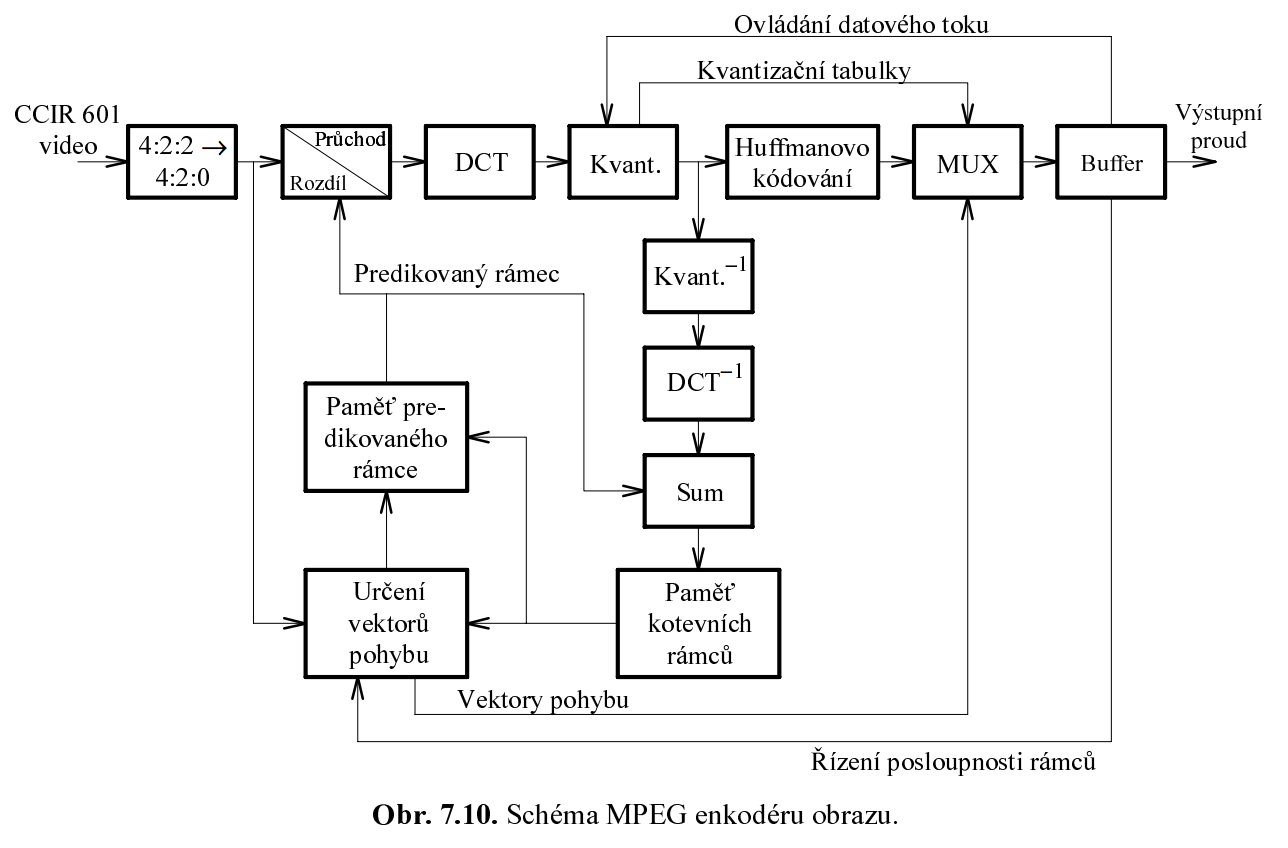
\includegraphics[width=\textwidth]{assets/7_mpeg_schema}
\end{figure}

\subsection{Principy úprav obrazu v prostorové a frekvenční doméně}
Úpravy nad obrazy lze provádět v \textbf{prostorové} (obraz je reprezentován souřadnicemi x, y a hodnotou pixelu) nebo \textbf{frekvenční} (snímek je popsán harmonickými funkcemi (sin a cos) různé amplitudy, frekvence a fáze) doméně. Většina operací nad prostorem signálů je popsána \textbf{operátorem}, pro převod do frekvenční domény se poté používá \textbf{(Diskrétní) Fourierova transformace}.

\begin{figure}[H]
	\centering
	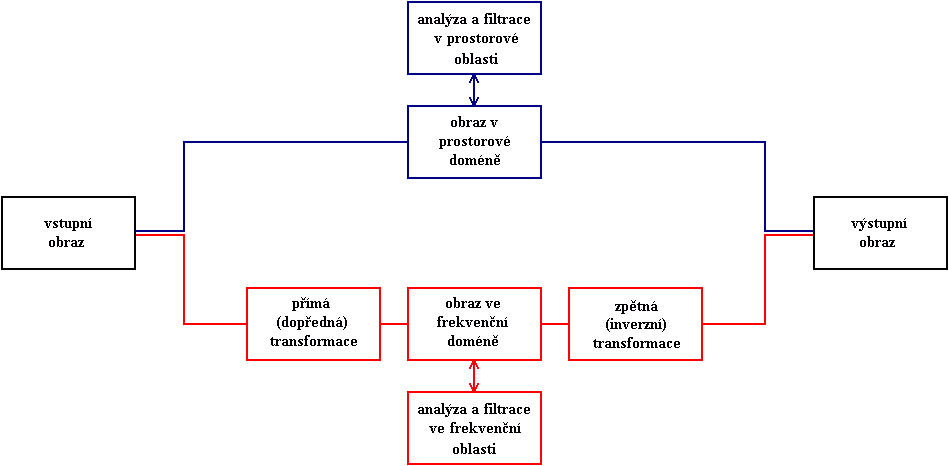
\includegraphics[width=0.8\textwidth]{assets/7_signaly}
\end{figure}

\subsection{Operace nad prostorem signálů}
\begin{itemize}
\item \textbf{Lineární operace} -- úprava signálu je popsána operátorem $\mathcal{O}$, velmi často předpokládáme, že operátor $\mathcal{O}$ má nějaké speciální vlastnosti. Platí: $\mathcal{O}\{af(x, y) + bg(x, y)\} = a\mathcal{O}\{f(x, y)\} + b\mathcal{O}\{g(x, y)\}$.
\item \textbf{Operace invariantní vůči posuvu} -- považujeme aby měl operátor kromě linearity ještě další vlastnosti (invarianci vůči posuvu). Operátor $\mathcal{O}$ je invariantní vůči posuvu, pokud pro všechna $f(x, y)$ platí: $g(x - a, y -b) = \mathcal{O}\{f(x-a, y-b)\}$. Méně formálně: pokud provedeme operátor na dva vzájemně posunuté ale jinak shodné signály, jejich výsledek bude také vzájemně posunutý ale jinak \textbf{stejný}.
\item \textbf{Dirakův impulz} -- je impulzová funkce $\delta(x, y) = 0$, v bodě (0, 0) je hodnota \textbf{nekonečno}, všude jinde nulovou, přičemž platí $\delta(-x, -y) = \delta(x, y)$, a \textbf{integrál} přes celou funkci je roven 1. JInak řečeno se jedná o funkci, která je nekonečně vysoká a nekonečně úzká v bodě (0, 0).
\end{itemize}

\subsection{Konvoluce (lineární sumace bodových zdrojů)}
Konvoluce představuje základní matematický \textbf{operátor}, který pracuje s dvěma funkcemi (značí se $*$). Umožňuje zpracování obrazových signálů jak v prostorové tak frekvenční doméně (konvoluční teorém). Spojitá konvoluce je definována takto:
\begin{equation*}
f(x, y) * h(x, y) = \int_{-\infty}{\infty}^{-\infty}{\infty} h(a, b) f(x - , y - b)dadb,
\end{equation*}
kde funkci $h$ nazýváme \textbf{konvoluční jádro} (filtr), přesně řečeno se jedná o impulzovou charakteristiku filtru. Při výpočtu se funkce $h$ v rovině $x, y$ otočí o $180^\circ$ (důsledek členů se zápornými znaménky). Konvoluční operátor má tyto \textbf{vlastnosti}:
\begin{itemize}
\item \textbf{Komutativní} -- $f * g = g * f$.
\item \textbf{Asociativní} -- $f * (g * h) = (f * g) * h$.
\item \textbf{Distributivní} -- $f * (g + h) = (f * g) + (f * h)$.
\item \textbf{Existence jednotky} -- $f * \delta = \delta * f = f$, kde $\delta$ je dirakův impulz a $\delta(x) = 0, x \neq 0$.
\item \textbf{Asociativita při násobení skalárem} -- $a(f * g) = (af) * g = f * (ag)$
\item \textbf{Konvoluční teorém} -- $\mathcal{F}(f * g) = [\mathcal{F}(f)] \cdot [\mathcal{F}(g)] = F \cdot G$, kde $\mathcal{F}[f(x)]$ značí Fourierovu transformaci. Jinými slovy: Fourierovým obrazem konvoluce funkcí $f, g$ je součin jejich Fourierových obrazů $F$ a $G$.
\end{itemize}

\subsubsection{Diskrétní konvoluce}
V počítačové grafice využíváme často pro zpracování dvourozměrného diskrétního signálu, je popsaná tímto vzorcem:
\begin{equation*}
(f*h)(x,y)=\sum _{{i=-k}}^{k}\sum _{{j=-k}}^{k}f(x-i,y-j)\cdot h(i,j)
\end{equation*}

V případě diskrétní konvoluce lze jádro chápat jako \textbf{tabulku} (konvoluční masku), kterou přiložíme na příslušné místo obrazu. Každý pixel překrytý tabulkou vynásobíme koeficientem v příslušné buňce a hodnoty sečteme, ty uložíme na pozici středového pixelu. V případě, že koeficienty již nejsou normalizované, je nutné je \textbf{normalizovat} (zprůměrovat), např.: maska $3 \times 3$ pokud je všude 1 (uniformní filtr) tak výsledek je nutné vydělit $9$.

Hodnoty konvoluční masky mají vliv na výsledek operace, používají se masky pro: \textbf{rozostření}, \textbf{zostření}, \textbf{detekci hran}, atd.

\begin{figure}[H]
	\centering
	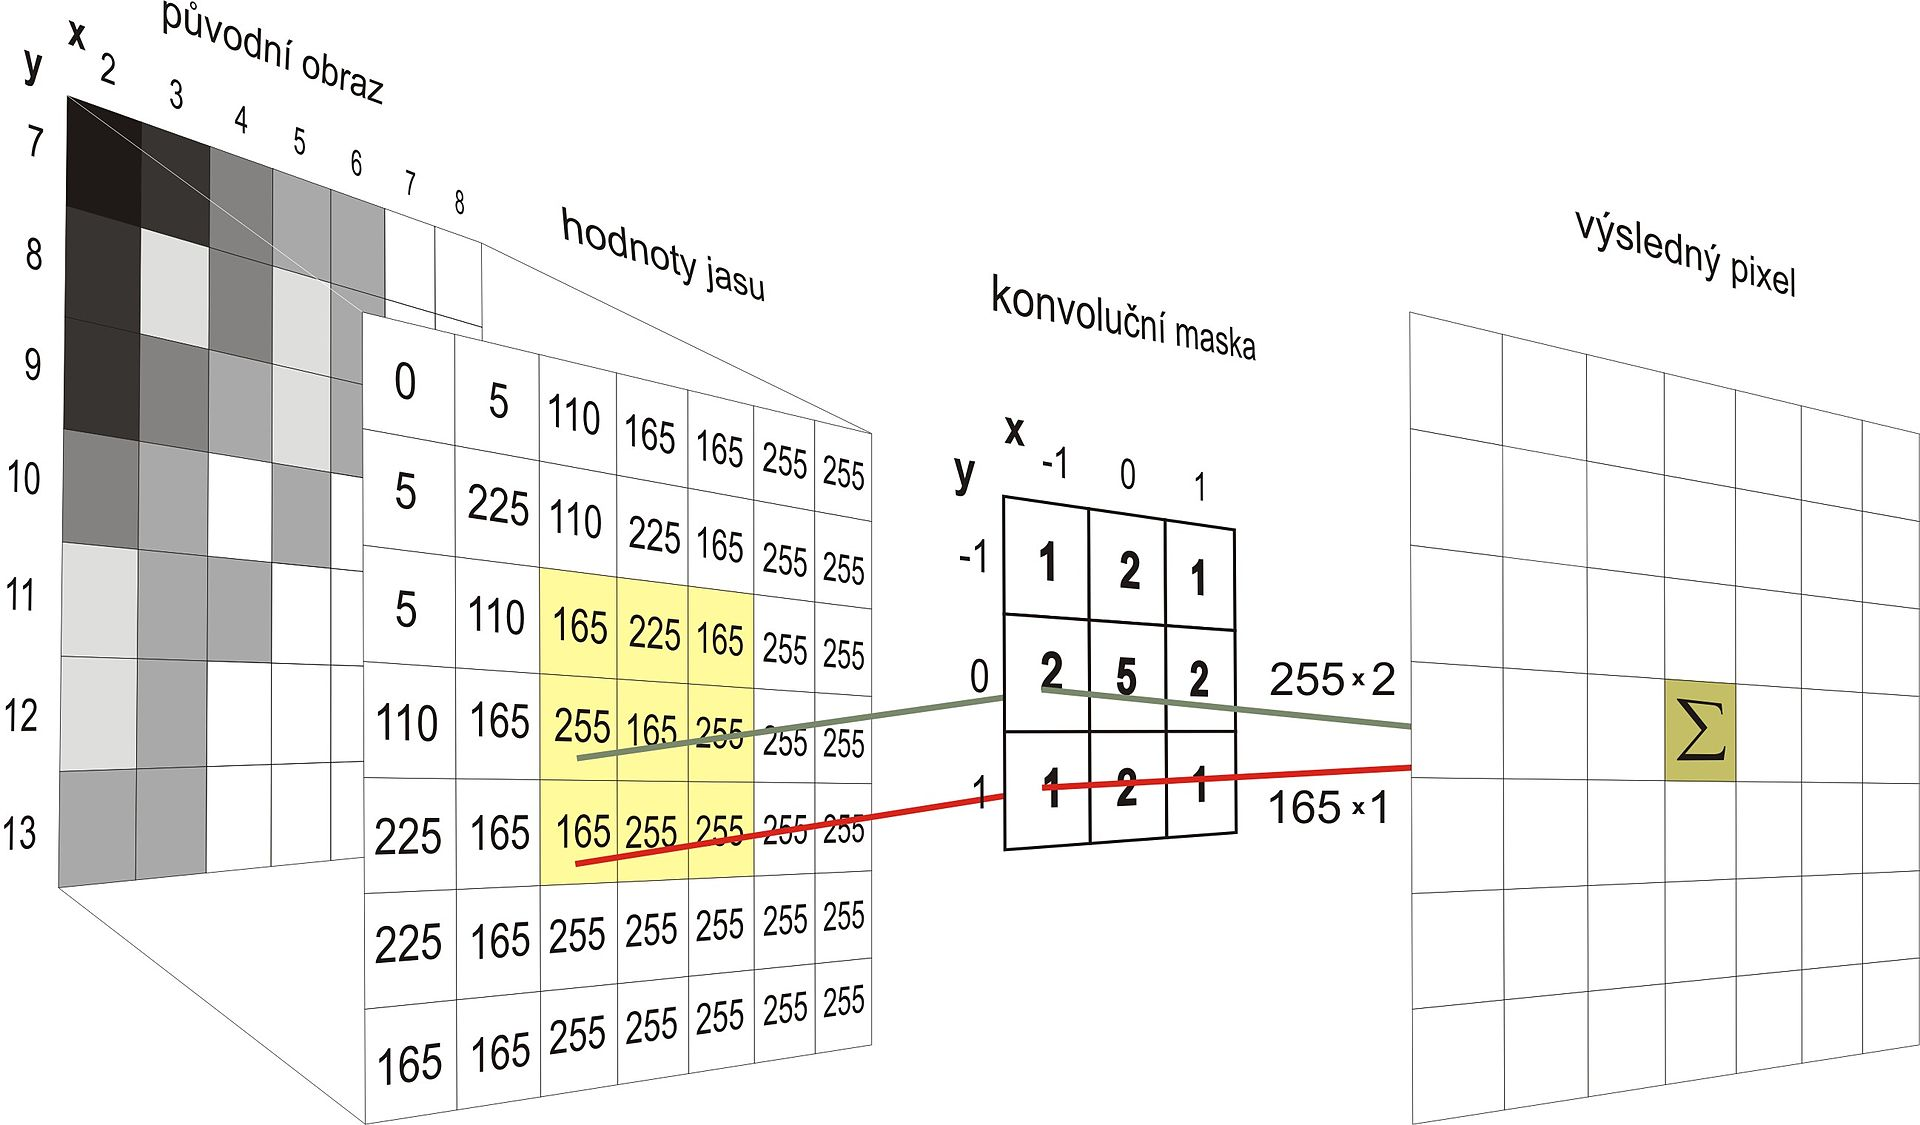
\includegraphics[width=0.7\textwidth]{assets/7_konvoluce}
\end{figure}

\subsection{Fourierova transformace}
Slouží pro převod obrazových signálů z prostorové do \textbf{frekvenční domény} (na komponenty složené ze sínů a cosínů). Pro analýzu \textbf{diskrétního} obrazu se využívá DFT, která je dána vztahem:
\begin{equation*}
F(k, l) = \sum_{m = 0}^{M - 1}\sum_{n = 0}^{N - 1} f(m, n) \frac{1}{\sqrt{MN}} \exp \left[ -j2\pi \left( \frac{mk}{M} + \frac{nl}{N} \right) \right],
\end{equation*}

kde $k = 0, \ldots M - 1$, $l = 0, \ldots N - 1$. Symbol $F(k, l)$ značí frekvenční spektrum obrazu s souřadnicemi $(k, l)$, které nabývá hodnot od 0 - $(M, N)$. Frekvenční spektrum obsahuje \textbf{komplexní čísla}, proto se pro zpracování obrazového signálu ve frekvenční oblasti používají \textbf{amplitudy} komplexních čísel (amplitudová frekvenční charakteristika) nebo výkonová spektrální hustota (koeficienty násobené komplexně sdruženým číslem). Příklad amplitudové charakteristiky je na následujícím obrázku.

\begin{figure}[H]
	\centering
	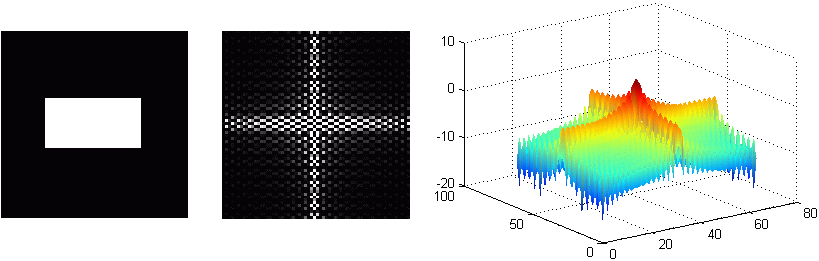
\includegraphics[width=0.9\textwidth]{assets/7_amp_ftt}
\end{figure}

Tato frekvenční charakteristika obsahuje \textbf{koeficienty odpovídající různým frekvenčním složkám}. Analýzou a operacemi s koeficienty ve frekvenční oblasti lze \textbf{modifikovat obraz v prostorové oblasti} např. realizovat filtr typu \textbf{dolní propust pro vyhlazení obrazu}. Pro získání modifikovaného obrazu je třeba převést koeficienty zpět do prostorové oblasti. Tomuto procesu se říká zpětná nebo někdy \textbf{inverzní Fouriérova transformace} IFT, jejíž diskrétní varianta IDFT je dána následujícím definičním vztahem:
\begin{equation*}
f(m, n) = \sum_{m = 0}^{M - 1}\sum_{n = 0}^{N - 1} F(k, l) \frac{1}{\sqrt{MN}} \exp \left[ j2\pi \left( \frac{mk}{M} + \frac{nl}{N} \right) \right].
\end{equation*}

\subsection{Filtrace ve frekvenční oblasti}
\textbf{Postup filtrace} obrazů ve frekvenční doméně je následující:
\begin{enumerate}
\item aplikace diskrétní Fourierovy transformace (DFT) $f(x, y) \rightarrow F(u, v)$,
\item aplikace filtru $G(u, v) = H(u, v) F(u, v)$, kde:
\begin{itemize}
\item $G(u, v)$ \ldots výslední snímek
\item $H(u, v)$ \ldots funkce filtrace (konvoluční maska?)
\item $F(u, v)$ \ldots původní snímek
\end{itemize}
inverzní Fourierova transformace (IDFT) $G(u, v) \rightarrow g(x, y)$.
\end{enumerate}

\subsubsection{Nízkofrekvenční, pásmový, vysokofrekvenční filtr}
Bázové funkce jsou síny a cosíny s rostoucí frekvencí. Tedy $ F(0, 0) $ (\textbf{střed obrázku}) reprezentuje DC složku, tedy \textbf{průměrný jas} napříč obrazem a $F(M -1, N - 1)$ reprezentuje \textbf{nejvyšší frekvenci}, to lze pozorovat na amplitudové charakteristice výše. 

Tedy \textbf{čím dále od středu, tím je frekvence vyšší}. Zároveň můžeme vidět, že \textbf{amplituda je menší pro vyšší frekvence}, nízké frekvence tedy obsahují více informací o obraze než ty vyšší a obecně se jich ve většině obrazů nachází více (čím rychlejší změna jasu/gradient tím vyšší frekvence). Všech těchto znalostí můžeme využít k návrhu požadovaného filtru:
\begin{itemize}
\item \textbf{Nízkofrekvenční} (lowpass) filtr může například propouštět pouze frekvence kolem středu (tedy ty nízké) a ostatní vynulujem, tento filtr lze navrhnout pomocí binární masky (bílý kruh ve středu) $\rightarrow$ \textbf{minimalizujeme ostré hrany}.
\item \textbf{Vysokofrekvenční} (highpass) filtr, postup je analogický k předchozímu, pouze tentokrát vynulujeme frekvence na středu a ty na krajích (vysoké) propustíme $\rightarrow$ \textbf{zvýrazníme hrany}.
\item \textbf{Pásmový} filtr propouští pouze předem definované pásmo.
\end{itemize}

\subsubsection{Butterworthův filtr}
Často se pro filtraci ve frekvenční oblasti využívá Butterworthův filtr, který má ze všech běžných filtrů (Gaussian, Chebyshev, Bessel) \textbf{nejméně zvlněné frekvenční spektrum} a konverguje k nule u maximální frekvence. Je dán vztahem:
\begin{equation*}
H(u, v) = \frac{1}{1 + \left( \frac{D(u, v)}{D_0} \right)^{\frac{2}{n}}}, \quad \textrm{kde } D(u, v)=\sqrt{(u - u_c)^2 + (v - v_c)^2}
\end{equation*}
kde $d(x, y)$ představuje běženě používanou L2-normu a $n$ je řád filtru (nejčastěji 1 nebo 2).

\begin{figure}[H]
	\centering
	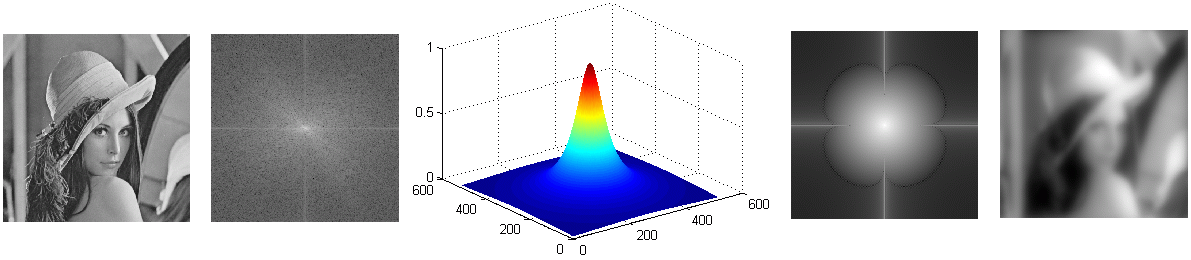
\includegraphics[width=\textwidth]{assets/7_ftt_filtery}
\end{figure}